\section{Phân hoạch không gian an toàn}
\label{sec:space_decomp}

Thay vì tiếp cận bài toán tránh vật cản theo cách truyền thống là mô tả các ràng buộc không lồi dựa trên bề mặt vật cản, ta chuyển đổi không gian cấu hình tự do $\mathcal{C}_{\mathrm{free}}$ thành hợp của một tập hữu hạn các vùng lồi bị chặn. Trong mô hình này, các vùng lồi có thể chồng lấn lên nhau, và bài toán hoạch định chuyển động được phát biểu lại dưới dạng một chương trình quy hoạch lồi nguyên hỗn hợp (Mixed-Integer Convex Program -- MICP). Các biến nguyên được sử dụng để gán từng đoạn quỹ đạo vào các vùng lồi an toàn tương ứng; số lượng biến nguyên chỉ phụ thuộc vào số lượng vùng trong phân hoạch -- không phụ thuộc vào số mặt của vật cản. Nhờ đó phương pháp giải quyết hiệu quả các môi trường phức tạp với hàng trăm vật cản. Hơn nữa, việc ràng buộc quỹ đạo nằm trọn trong các vùng lồi đảm bảo tính an toàn liên tục theo thời gian.

Để giải quyết thách thức tính toán của bước phân hoạch, một số phương pháp đã được phát triển. Dưới đây là ba phương pháp được sử dụng trong đồ án này:

\subsection{Phân hoạch Lồi Xấp xỉ (ACD)}

Phương pháp Approximate Convex Decomposition (ACD) giới thiệu một cách tiếp cận khác biệt để quản lý sự phức tạp của không gian phi lồi. Thay vì yêu cầu tính lồi hoàn hảo, ACD cho phép các thành phần \textit{lồi xấp xỉ} trong một dung sai do người dùng xác định $\tau$~\cite{LienAmato2006}. Điều này thường dẫn đến các phân hoạch có ít thành phần hơn nhiều và phù hợp hơn với các đặc điểm cấu trúc nổi bật của hình học.

\subsubsection{Các Khái niệm Cơ bản trong Phân hoạch Lồi}
\label{subsubsec:acd_basic_concepts}

Phần này trình bày các khái niệm hình học cơ bản được sử dụng trong quá trình phân hoạch đa giác không lồi thành các vùng lồi.
Các định nghĩa này đóng vai trò nền tảng cho các phương pháp đo độ lõm và các thuật toán phân hoạch ở các phần sau.

\begin{enumerate}
    \item \textbf{Bao lồi (Convex Hull -- $H_P$):}
    Bao lồi của một đa giác $P$ là \textbf{tập hợp lồi nhỏ nhất chứa toàn bộ đa giác} đó.
    Trực quan, có thể hình dung bao lồi như một sợi dây chun được kéo căng bao quanh đa giác.
    Một đa giác $P$ được gọi là \textbf{lồi} nếu và chỉ nếu nó trùng với bao lồi của chính nó:
    \[
    P = H_P.
    \]

    \item \textbf{Đỉnh lõm (Notch):}
    Là các đỉnh của đa giác $P$ \textbf{không nằm trên bao lồi} $H_P$.
    Về mặt hình học, đây là những đỉnh có \textbf{góc trong lớn hơn $180^\circ$}.
    Các đỉnh lõm biểu hiện các đặc trưng lõm (concave features) trên biên của đa giác.

    \item \textbf{Cầu (Bridge):}
    Là các cạnh của bao lồi $\partial H_P$ nối hai đỉnh không liền kề của biên ngoài $\partial P_0$.
    Tập hợp các cầu được định nghĩa:
    \[
    \text{BRIDGES}(P) = \partial H_P \setminus \partial P.
    \]
    Mỗi cầu ``bắc qua'' một vùng lõm của đa giác.

    \item \textbf{Túi (Pocket):}
    Là các \textbf{chuỗi cạnh liên tiếp} của biên đa giác $\partial P$ không thuộc bao lồi $\partial H_P$:
    \[
    \text{POCKETS}(P) = \partial P \setminus \partial H_P.
    \]
    Mỗi túi tương ứng với một ``vịnh lõm'' (concave bay) trên đường biên của đa giác.
\end{enumerate}

\begin{figure}[H]
    \centering
    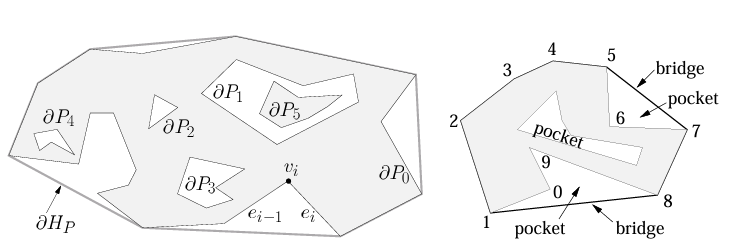
\includegraphics[width=0.7\linewidth]{experiments/image/ACD-5.png}
    \caption[Các khái niệm cơ bản trong phân hoạch lồi]{Minh họa bao lồi $H_P$, đỉnh lõm (notch), cầu (bridge) và túi (pocket) của một đa giác không lồi $P$.}
    \label{fig:acd_basic_concepts}
\end{figure}

\subsubsection{Ý tưởng và Chi tiết Thuật toán}

Thuật toán ACD là một chiến lược chia để trị đệ quy~\cite{LienAmato2006}:
\begin{enumerate}
\item \textbf{Đo độ lõm:} Xác định đỉnh lõm quan trọng nhất trong đa giác -- đỉnh có độ lõm lớn nhất. Các thước đo độ lõm khác nhau sẽ được trình bày ở mục~\ref{subsubsec:concavity_measures}.

\item \textbf{Kiểm tra dung sai:} Nếu độ lõm tối đa nhỏ hơn $\tau$, quá trình kết thúc đối với thành phần đó.

\item \textbf{Giải quyết đỉnh lõm:} Nếu độ lõm vượt $\tau$, một đường cắt được thêm vào để giải quyết đỉnh lõm, chia đa giác thành hai thành phần mới (hoặc hợp nhất một lỗ).

\begin{figure}[H]
    \centering
    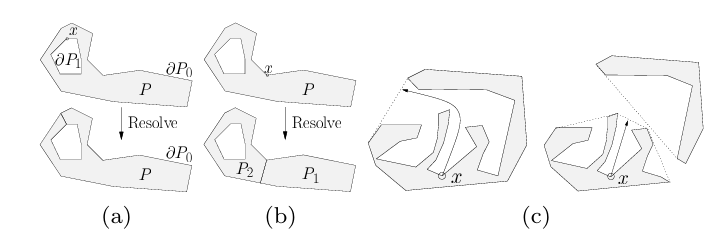
\includegraphics[width=1\linewidth]{experiments/image/ACD-3.png}
    \caption[Ví dụ ACD]{%
        (a) Nếu $x \in \partial P_i$ với $i > 0$ (biên của lỗ), hàm \texttt{Resolve} \textbf{gộp} lỗ $P_i$ vào đa giác ngoài $P_0$.
        (b) Nếu $x \in \partial P_0$ (biên ngoài), hàm \texttt{Resolve} \textbf{tách} đa giác $P$ thành hai thành phần $P_1$ và $P_2$.
        (c) \textbf{Độ lõm} tại điểm $x$ thay đổi sau khi đa giác được phân hoạch.%
    }
\end{figure}

\item \textbf{Đệ quy:} Quá trình được áp dụng đệ quy cho các thành phần mới.

\begin{figure}[H]
    \centering
    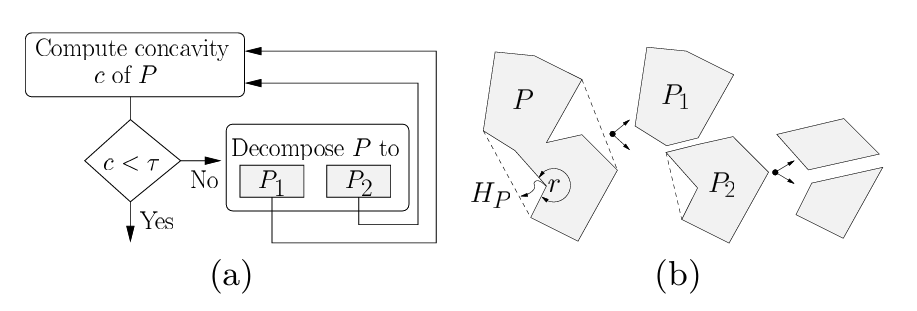
\includegraphics[width=1\linewidth]{experiments/image/ACD-1.png}
    \caption[Mô tả quá trình đệ quy ACD]{Quá trình đệ quy tiếp tục cho đến khi đạt đến giới hạn dung sai $\tau$ do người dùng đặt trước.}
\end{figure}

\end{enumerate}

\subsubsection{Các Thước đo Độ lõm}
\label{subsubsec:concavity_measures}

Chất lượng của phân hoạch phụ thuộc rất nhiều vào \textbf{cách đo độ lõm} của các đỉnh trong đa giác không lồi. Các phương pháp đo độ lõm phổ biến bao gồm:

\begin{enumerate}
    \item \textbf{Độ lõm Đường thẳng (Straight-Line Concavity -- SL-Concavity)}:
    Là khoảng cách Euclid từ một đỉnh trong \textit{túi} (pocket) đến \textit{cầu} (bridge) liên kết của nó.
    Phương pháp này rất nhanh, nhưng \textbf{không đảm bảo tính đơn điệu}, có thể khiến một số đặc trưng lõm quan trọng bị bỏ sót.

    \begin{figure}[H]
        \centering
        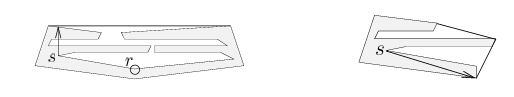
\includegraphics[width=1\linewidth]{experiments/image/ACD-2.png}
        \caption[Trường hợp không đảm bảo tính đơn điệu của SL-Concavity]{%
            Giả sử $r$ là đỉnh lõm có độ lõm lớn nhất.
            Sau khi giải quyết $r$, độ lõm của $s$ tăng lên.
            Nếu $\mathrm{concavity}(r) < \tau$, đỉnh $s$ sẽ không bao giờ được xử lý,
            ngay cả khi $\mathrm{concavity}(s) > \tau$.%
        }
        \label{fig:nonmonotonic-concavity}
    \end{figure}

    \item \textbf{Độ lõm Đường đi Ngắn nhất (Shortest Path Concavity -- SP-Concavity)}:
    Là \textbf{chiều dài đường đi ngắn nhất} từ một đỉnh trong túi đến cầu tương ứng, với điều kiện đường đi phải nằm hoàn toàn trong túi.
    Phương pháp này chậm hơn SL-Concavity nhưng \textbf{đảm bảo tính đơn điệu}: độ lõm của các đỉnh giảm dần sau mỗi lần phân hoạch,
    giúp đảm bảo tất cả các đặc trưng lõm vượt ngưỡng $\tau$ đều được xử lý.

    \item \textbf{Độ lõm Lai (Hybrid Concavity -- H-Concavity)}:
    Một giải pháp trung gian thực tiễn: sử dụng SL-Concavity nhanh làm mặc định và chỉ chuyển sang SP-Concavity khi \textbf{phát hiện khả năng không đơn điệu}. Bước kiểm tra dựa trên so sánh pháp tuyến $n_\beta$ của cầu và pháp tuyến $n_i$ của đỉnh trong túi: nếu $n_i \cdot n_\beta < 0$, biên túi bị đảo hướng -- dấu hiệu của túi phức tạp mà SL-Concavity có thể thất bại.

    \begin{figure}[H]
        \centering
        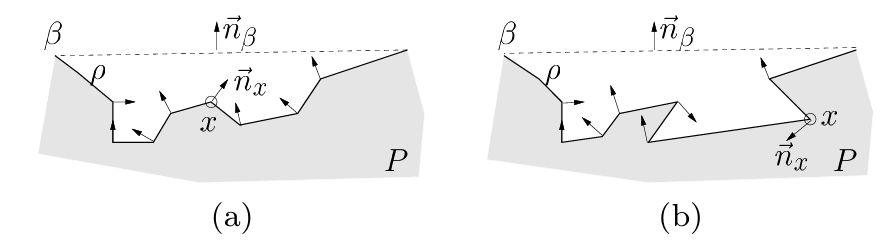
\includegraphics[width=1\linewidth]{experiments/image/ACD-6.png}
        \caption[Độ lõm Lai (Hybrid Concavity -- H-Concavity)]{SL-Concavity xử lý chính xác túi (a) vì không có pháp tuyến đỉnh nào trong túi ngược chiều pháp tuyến cầu. Tuy nhiên, túi (b) có thể dẫn đến độ lõm giảm không đơn điệu, khiến SL-Concavity thất bại.}
    \end{figure}

\end{enumerate}


\subsection{Iterative Regional Inflation by Semidefinite Programming (IRIS)}

Thay vì cố gắng bao phủ toàn bộ không gian tự do cùng một lúc, thuật toán IRIS (Iterative Regional Inflation by Semidefinite Programming) đặt ra câu hỏi: \textit{``Với một điểm mầm (seed) cho trước, đa diện lồi lớn nhất không va chạm với bất kỳ vật cản nào xung quanh nó là gì?''} Mỗi lần gọi thuật toán cho ra một đa diện lồi từ một điểm mầm duy nhất; để phủ toàn bộ $\mathcal{C}_{\mathrm{free}}$, thuật toán được chạy nhiều lần với các điểm mầm khác nhau.

\subsubsection{Ý tưởng và Chi tiết Thuật toán}

IRIS là một quy trình tối ưu hóa lặp gồm bốn bước:
\begin{enumerate}
\item \textbf{Khởi tạo}: Thuật toán tạo một ellipsoid ban đầu là hình cầu rất nhỏ có tâm tại điểm mầm.

\item \textbf{Tìm Siêu phẳng Phân cách (QP)}:

\begin{figure}[!htp]
    \centering
    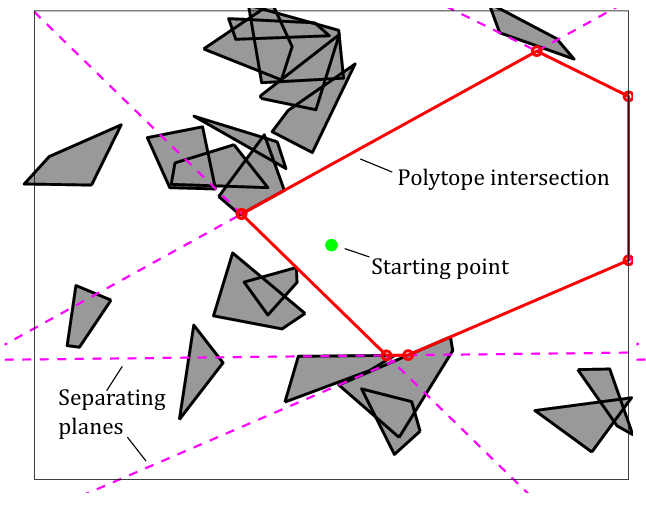
\includegraphics[width=0.5\linewidth]{experiments/image/iris_algo_1.png}
    \caption{Minh họa siêu phẳng phân cách ellipsoid khỏi các vật cản trong IRIS.}
\end{figure}

Đối với ellipsoid hiện tại, thuật toán tìm điểm gần nhất trên mỗi vật cản, sau đó xây dựng siêu phẳng phân cách ellipsoid khỏi các vật cản đó. Mỗi siêu phẳng tiếp tuyến với ellipsoid được mở rộng và đi qua điểm gần nhất trên vật cản tương ứng. Các siêu phẳng thừa (không xác định biên của vùng lồi kết quả) được loại bỏ để giữ quy mô bài toán nhỏ. Bước này gồm bốn thao tác nhỏ:

\begin{description}
    \item[1.] \textbf{Biến đổi về không gian cầu đơn vị}: Việc tính khoảng cách đến ellipsoid phức tạp hơn so với cầu đơn vị. Ellipsoid $E$ được định nghĩa là ảnh của cầu đơn vị qua phép biến đổi affine $x = C\tilde{x} + d$ (với $C$ xác định hình dạng và hướng, $d$ là tâm). Áp dụng phép biến đổi ngược $\tilde{x} = C^{-1}(x - d)$ để đưa mọi điểm về không gian cầu đơn vị; khi đó mỗi vật cản $l_j$ được biến đổi thành $\tilde{l}_j$.

    \item[2.] \textbf{Tìm điểm gần nhất bằng Quy hoạch Toàn phương (QP)}: Tìm điểm trên vật cản $l_j$ gần ellipsoid $E$ nhất tương đương với tìm điểm trên $\tilde{l}_j$ gần gốc tọa độ nhất:
    \[
    \begin{aligned}
        &\underset{\tilde{x} \in \mathbb{R}^n,\, w \in \mathbb{R}^m}{\text{minimize}} && \|\tilde{x}\|^2 \\
        &\text{subject to}
        &&
        \begin{cases}
            \begin{bmatrix} \tilde{v}_{j,1} & \tilde{v}_{j,2} & \cdots & \tilde{v}_{j,m} \end{bmatrix} w = \tilde{x}, \\
            \sum_{i=1}^{m} w_i = 1, \\
            w_i \ge 0, \quad i = 1,\dots,m.
        \end{cases}
    \end{aligned}
    \]
    Về bản chất, ta tìm \textbf{tổ hợp lồi} của các đỉnh đã biến đổi $\tilde{v}_{j,k}$ gần gốc tọa độ nhất.

    \item[3.] \textbf{Xây dựng siêu phẳng tiếp tuyến}: Sau khi tìm được điểm $x^*$ gần nhất, siêu phẳng tiếp tuyến với ellipsoid tại $x^*$ được xây dựng. Ellipsoid có dạng $E = \{x \mid (x - d)^{\top} C^{-1} C^{-\top} (x - d) \le 1\}$, nên pháp tuyến tại $x^*$ là:
    \[
    a_j = 2C^{-1}C^{-\top}(x^* - d), \qquad b_j = a_j^{\top}x^*.
    \]
    Siêu phẳng $a_j^{\top}x = b_j$ được thêm vào như một ràng buộc tuyến tính, đảm bảo ellipsoid mở rộng không giao với vật cản tương ứng.

    \item[4.] \textbf{Lặp lại với tất cả vật cản}: Thu được tập siêu phẳng xác định một đa diện lồi (polytope) không giao với bất kỳ vật cản nào.
\end{description}

\item \textbf{Tìm Ellipsoid Nội tiếp Cực đại (SDP)}: Giao của các nửa không gian từ bước~2 tạo thành một đa diện lồi $P = \{x \in \mathbb{R}^n \mid Ax \leq b\}$. Thuật toán sau đó tìm ellipsoid có thể tích lớn nhất nội tiếp trong $P$.

\begin{figure}[!htp]
    \centering
    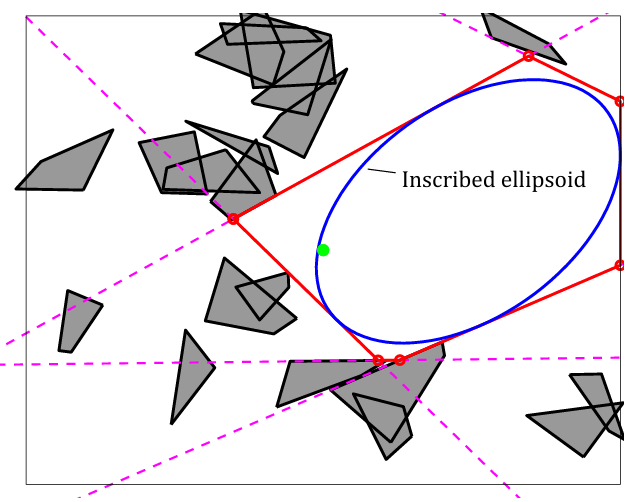
\includegraphics[width=0.5\linewidth]{experiments/image/iris_2.png}
    \caption{Ellipsoid nội tiếp cực đại trong đa diện lồi hiện tại.}
\end{figure}

Ellipsoid được tham số hóa là $\mathcal{E} = \{C\tilde{x} + d \mid \|\tilde{x}\|_2 \leq 1\}$ với thể tích tỉ lệ $\det(C)$. Bài toán tối ưu lồi tương ứng là:
\begin{equation}
\begin{aligned}
    \underset{C,d}{\text{maximize}} \quad & \log \det C \\
    \text{subject to} \quad & \|a_i^{\top} C\|_2 + a_i^{\top} d \leq b_i, \quad \forall i = 1, \ldots, N, \\
    & C \succ 0.
\end{aligned}
\end{equation}
Ràng buộc $\|a_i^{\top}C\|_2 + a_i^{\top}d \le b_i$ đảm bảo mọi điểm của ellipsoid đều nằm trong $P$. Đây là bài toán bán xác định dương (SDP), có thể giải hiệu quả bằng các bộ giải SDP chuẩn.

\noindent\textbf{Mục tiêu:} Cực đại hoá $\log \det C$ để tối đa hoá thể tích ellipsoid. \\[2pt]
\noindent\textbf{Ràng buộc:} Đảm bảo mọi điểm của ellipsoid đều nằm trong đa diện $P$.

\item \textbf{Lặp lại}: Ellipsoid mới, lớn hơn được sử dụng làm điểm khởi đầu cho vòng lặp tiếp theo. Quá trình hội tụ khi thể tích ellipsoid ngừng tăng đáng kể, trả về một đa diện lồi cùng ellipsoid nội tiếp của nó.
\end{enumerate}

\begin{figure}[!htp]
    \centering
    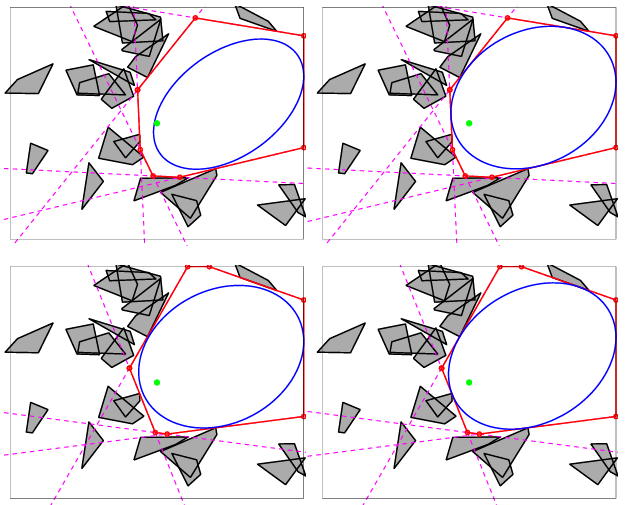
\includegraphics[width=0.6\linewidth]{experiments/image/iris-3.png}
    \caption[Vòng lặp IRIS]{Quá trình lặp IRIS hội tụ sau 4--8 vòng trong hầu hết trường hợp.}
\end{figure}

\subsubsection{Đặc tính của Thuật toán}

\begin{itemize}
\item \textbf{Loại thuật toán}: IRIS là phương pháp xấp xỉ để bao phủ không gian tự do. Một lần chạy chỉ tạo ra một vùng lồi; để phủ hoàn chỉnh $\mathcal{C}_{\mathrm{free}}$ cần chạy nhiều lần với các điểm mầm khác nhau.

\item \textbf{Độ phức tạp thời gian}: IRIS thường hội tụ qua 4--8 vòng lặp. Mỗi vòng gồm bước tìm siêu phẳng (QP, tăng tuyến tính theo số vật cản) và bước tìm ellipsoid nội tiếp (SDP, gần như không đổi nhờ loại siêu phẳng thừa).
\begin{figure}[!htp]
    \centering
    
\includegraphics[width=1\linewidth]{experiments/image/time-iris.png}
    \caption[Độ phức tạp thời gian của IRIS]{Độ phức tạp thời gian của IRIS~\cite{DeitsTedrake2014}.}
\end{figure}

\item \textbf{Xử lý vật cản không lồi}:

\textit{Trong không gian làm việc (workspace):} IRIS ban đầu giả định vật cản là lồi. Để xử lý vật cản không lồi, ta tiền xử lý bằng cách lấy bao lồi hoặc phân hoạch chúng thành các mảnh lồi trước khi chạy IRIS~\cite{DeitsTedrake2014}. Điều này khả thi vì IRIS mở rộng hiệu quả theo số lượng vật cản.

\textit{Trong không gian cấu hình (configuration space):} Đối với robot có động học phức tạp, các phần mở rộng như IRIS-NP~\cite{DeitsTedrake2023NP} và C-IRIS~\cite{DeitsTedrake2022CIRIS} được sử dụng để xử lý ràng buộc va chạm được định nghĩa ẩn và không lồi.

\end{itemize}


\subsection{Visibility Clique Cover (VCC)}
\label{subsec:vcc}

Thuật toán Visibility Clique Cover (VCC) giải quyết trực tiếp một hạn chế chính của IRIS: sự phụ thuộc vào chất lượng điểm mầm~\cite{DeitsTedrake2023VCC}. Việc lấy mầm ngẫu nhiên thường không hiệu quả. VCC tự động hóa quá trình này bằng cách trước tiên tìm hiểu cấu trúc toàn cục của không gian tự do, sau đó đặt điểm mầm có chủ đích vào các vùng có khả năng mở rộng lớn.

\subsubsection{Ý tưởng và Chi tiết Thuật toán}

\begin{figure}[!htp]
    \centering
    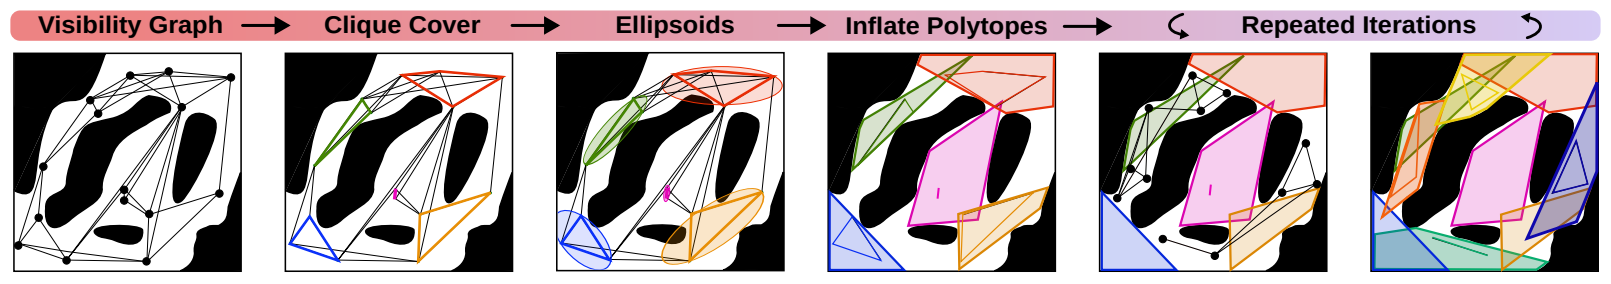
\includegraphics[width=1.0\linewidth]{experiments/image/VCC-pipeline.png}
    \caption[Tổng quan về Quy trình VCC]{Tổng quan về quy trình VCC~\cite{DeitsTedrake2023VCC}.}
    \label{fig:vcc_pipeline}
\end{figure}

Quy trình VCC như minh họa trong Hình~\ref{fig:vcc_pipeline} bao gồm năm bước chính:
\begin{enumerate}
\item \textbf{Lấy mẫu và xây dựng đồ thị khả kiến}: Thuật toán lấy mẫu $n$ điểm ngẫu nhiên trong $\mathcal{C}_{\mathrm{free}}$. Các điểm này tạo thành đỉnh của một đồ thị khả kiến (visibility graph)\footnote{\textit{Visibility graph} là đồ thị trong đó có cạnh nối hai đỉnh nếu và chỉ nếu đoạn thẳng nối chúng nằm hoàn toàn trong $\mathcal{C}_{\mathrm{free}}$, tức là không va chạm với bất kỳ vật cản nào.}.

% \begin{figure}[H]
%     \centering
%     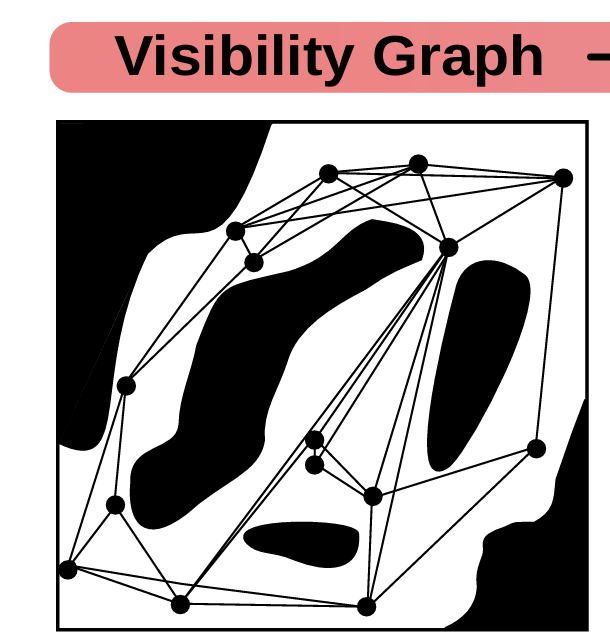
\includegraphics[width=0.5\linewidth]{experiments/image/VCC-1.png}
%     \caption{Lấy mẫu và xây dựng đồ thị khả kiến.}
% \end{figure}

\item \textbf{Tìm Clique Cover}: Thuật toán tìm một tập hợp các clique lớn (đồ thị con đầy đủ) trong đồ thị khả kiến. Ý tưởng cốt lõi: tập điểm mà tất cả đều ``nhìn thấy'' nhau có khả năng cao nằm trong cùng một vùng lồi\footnote{Nếu hai điểm nhìn thấy nhau, đoạn thẳng nối chúng nằm trong $\mathcal{C}_{\mathrm{free}}$ -- tính chất đặc trưng của tập lồi.}. Clique cover được tìm bằng thuật toán tham lam lặp lại, trong đó mỗi vòng lặp giải gần đúng bài toán MAXCLIQUE thường được xây dựng dưới dạng Integer Linear Programming (ILP).

% \begin{figure}[H]
%     \centering
%     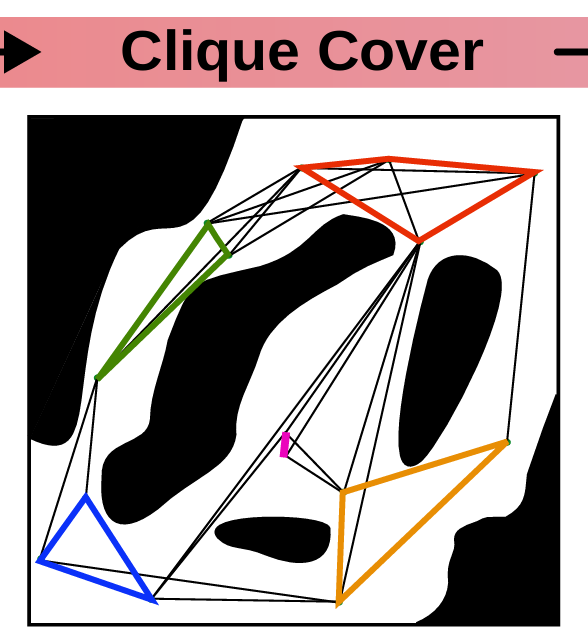
\includegraphics[width=0.5\linewidth]{experiments/image/VCC-2.png}
%     \caption{Tìm Clique Cover.}
% \end{figure}

\item \textbf{Khởi tạo Ellipsoid}: Với mỗi clique tìm được, thuật toán tính ellipsoid có thể tích nhỏ nhất bao quanh tất cả các điểm trong clique đó. Ellipsoid này cung cấp tâm (điểm mầm) và hình dạng ban đầu cho bước lấp đầy tiếp theo.

% \begin{figure}[H]
%     \centering
%     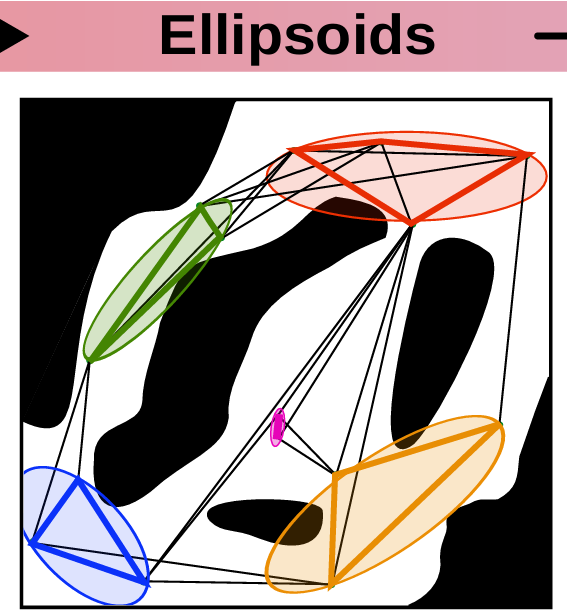
\includegraphics[width=0.5\linewidth]{experiments/image/VCC-3.png}
%     \caption{Khởi tạo Ellipsoid từ clique.}
% \end{figure}

\item \textbf{Lấp đầy thành Đa diện}: Tâm và hình dạng của mỗi ellipsoid khởi tạo một vòng lặp IRIS duy nhất. Nhờ ellipsoid đã được định hướng bởi hình học cục bộ, bước lấp đầy thường chỉ cần một vòng lặp -- hiệu quả hơn đáng kể so với IRIS tiêu chuẩn~\cite{DeitsTedrake2023VCC}.

% \begin{figure}[H]
%     \centering
%     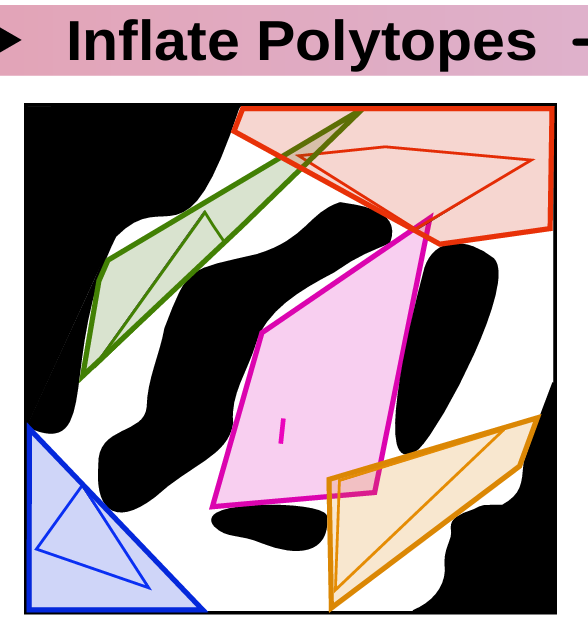
\includegraphics[width=0.45\linewidth]{experiments/image/VCC-4.png}
%     \caption{Lấp đầy thành đa diện lồi.}
% \end{figure}

\item \textbf{Lặp lại và hội tụ}: Quá trình được lặp lại bằng cách lấy mẫu mới từ không gian chưa được phủ cho đến khi đạt độ phủ mong muốn.

% \begin{figure}[H]
%     \centering
%     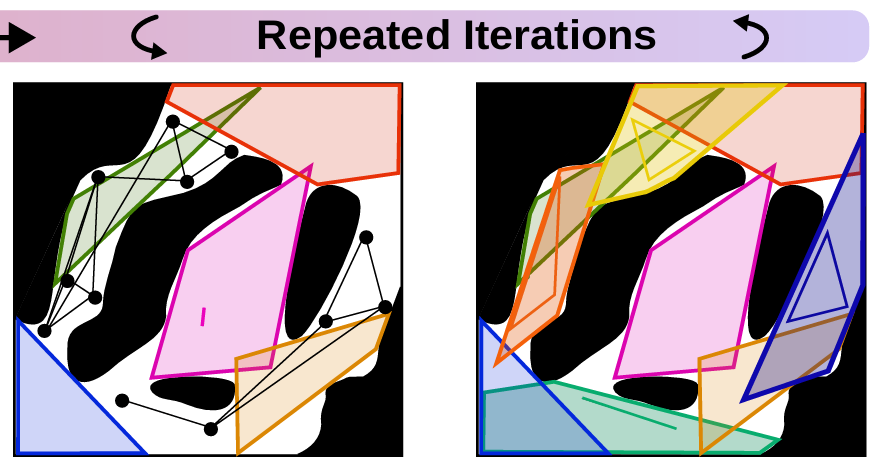
\includegraphics[width=1\linewidth]{experiments/image/VCC-5.png}
%     \caption{Quá trình lặp VCC.}
% \end{figure}

\end{enumerate}

\subsubsection{Đặc tính của Thuật toán}

\begin{itemize}
\item \textbf{Tự động hóa đặt điểm mầm}: Khác với IRIS yêu cầu lựa chọn điểm mầm thủ công, VCC tự suy ra vị trí đặt mầm từ cấu trúc đồ thị khả kiến, giảm thiểu sự phụ thuộc vào kiến thức chuyên gia về môi trường.

\item \textbf{Độ phức tạp tính toán}: Bài toán MAXCLIQUE là NP-hard trong trường hợp tổng quát; VCC dùng thuật toán tham lam lặp lại để giải gần đúng, cho kết quả tốt trong thực tế với thời gian đa thức đối với hầu hết cấu hình môi trường. Giai đoạn lấp đầy đa diện tương đương một vòng lặp IRIS với khởi tạo tốt, nên nhanh hơn IRIS tiêu chuẩn đáng kể.

\item \textbf{Chất lượng phân hoạch}: VCC có xu hướng tạo ít vùng hơn để phủ cùng một không gian so với IRIS lấy mầm ngẫu nhiên, nhờ điểm mầm được đặt có chủ đích dựa trên cấu trúc hình học. Tuy nhiên, chất lượng phụ thuộc vào số lượng mẫu $n$ và tính đại diện của đồ thị khả kiến.

\item \textbf{Giới hạn}: VCC yêu cầu lấy mẫu đủ dày để xây dựng đồ thị khả kiến đại diện. Trong các không gian hẹp (narrow passages) hoặc không gian chiều cao, đây có thể là thách thức đáng kể.
\end{itemize}

\subsection*{Tổng kết và lựa chọn phương pháp}

Ba phương pháp trình bày ở trên có những ưu nhược điểm bổ sung cho nhau, được tóm tắt trong Bảng~\ref{tab:decomp_comparison}.

\begin{table}[htbp]
\centering
\caption{So sánh các phương pháp phân hoạch không gian an toàn.}
\label{tab:decomp_comparison}
\begin{tabular}{lccc}
\hline
\textbf{Tiêu chí} & \textbf{ACD} & \textbf{IRIS} & \textbf{VCC} \\
\hline
Phủ toàn bộ $\mathcal{C}_{\mathrm{free}}$ & Có (xấp xỉ $\tau$) & Theo seed & Tự động lặp \\
Yêu cầu vật cản lồi & Không & Có & Có \\
Tự động đặt điểm mầm & -- & Không & Có \\
Bộ giải sử dụng & Heuristic & QP + SDP & ILP + QP + SDP \\
Phù hợp với & Polygon 2D & $\mathbb{R}^n$ tổng quát & $\mathbb{R}^n$ tổng quát \\
\hline
\end{tabular}
\end{table}

Trong đồ án này, bước phân hoạch không gian an toàn được thực hiện bằng một trong các phương pháp trên để tạo ra họ vùng lồi $\{Q_v\}$ làm đầu vào chung cho cả hai hướng tiếp cận GCS-Bézier (Phần~\ref{sec:gcs_approach}) và GCS-DMS (Phần~\ref{sec:ocp_dms_approach}). Chi tiết về tham số và kết quả phân hoạch trên các môi trường thực nghiệm được trình bày ở Chương~\ref{ch:experiments}.
